\section{Introduction}

\begin{figure}[t]
    \centerline{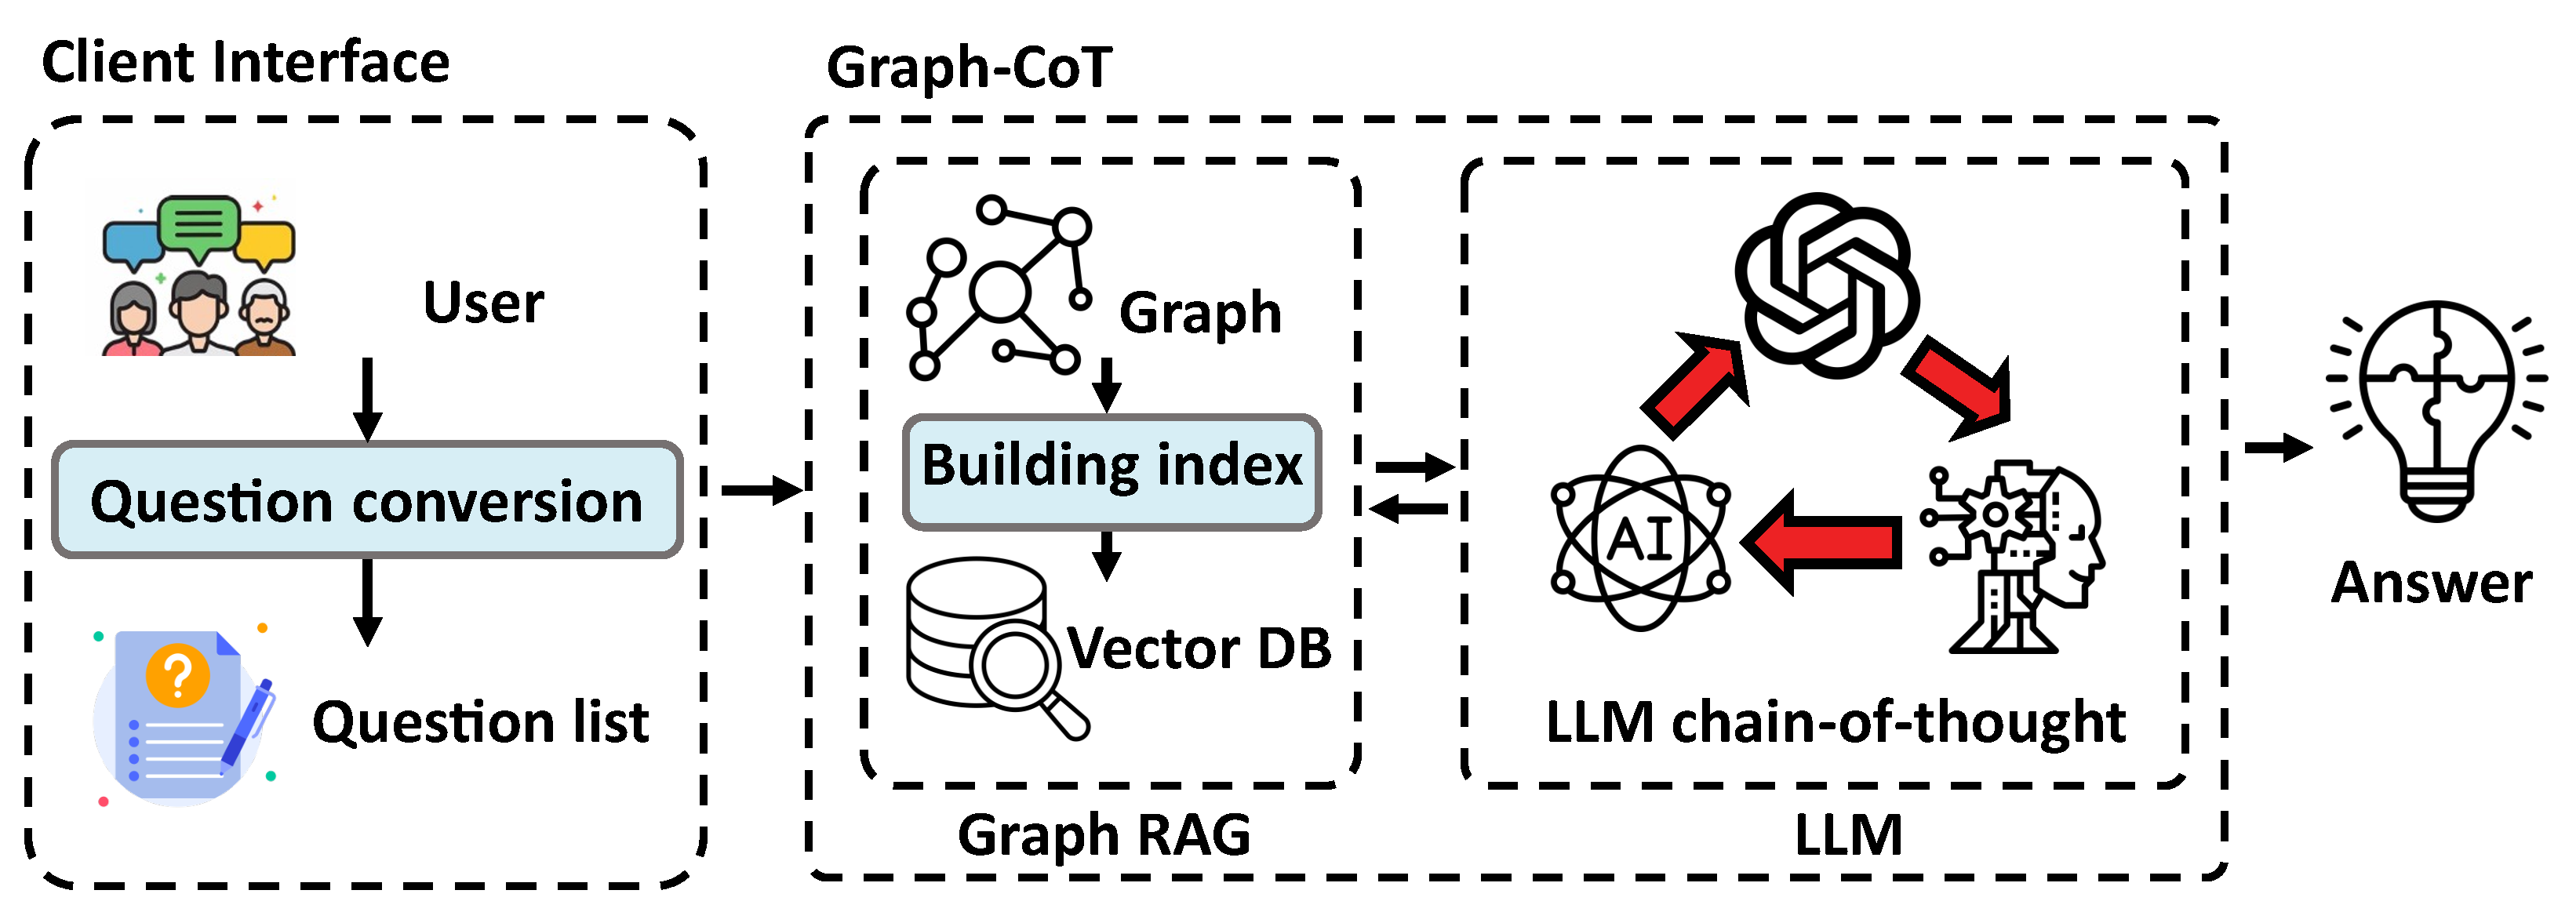
\includegraphics[width=1\linewidth]{figures/introduction.pdf}}
    \caption{Graph-CoT Framework.}
    \label{fig:introduction}
\end{figure}

Large Language Models (LLMs) such as GPT-4~\cite{achiam2023gpt}, Qwen~\cite{qwen}, Gemini~\cite{team2023gemini}, and DeepSeek~\cite{deepseekai2024deepseekv3technicalreport} have demonstrated remarkable general-purpose capabilities across multiple domains, including vibe coding~\cite{liu2023your,jiang2024self,jiang2024survey,zhang2023planning}, ChatBot~\cite{thoppilan2022lamda,hosseini2020simple,zhang2024comprehensive,yang2024zhongjing}, and complex reasoning~\cite{plaat2024reasoning,huang2022towards,lai2024lisa,lu2023chameleon}. 
%
In practice, reasoning ability and quality have become crucial determinants of the utility of LLMs for real-world applications such as program synthesis~\cite{gehring2024rlef,wang2023review}, robotic planning~\cite{zawalski2024robotic,cheng2024empowering}, and autonomous agents~\cite{deng2023mind2web,wang2024survey}.

To support complex reasoning, Chain-of-Thought (CoT) prompting~\cite{wei2022chain} has emerged as a core mechanism, enabling step-by-step inference by decomposing complex tasks into intermediate steps and thereby emulating human problem-solving processes.
%
Despite these advances, LLMs remain constrained by hallucination and limited access to domain-specific, proprietary, or real-time information. To mitigate these limitations, Retrieval-Augmented Generation (RAG)~\cite{lewis2020retrieval,guu2020retrieval,asai2024self} has become a widely adopted paradigm, enhancing factuality and grounding by integrating external retrieval into the generation process.


\stitle{Graph-CoT.}
Conventional RAG pipelines operate primarily on independent text chunks (i.e., flat text), overlooking the rich structural and relational dependencies across entities that are prevalent in real-world data such as knowledge graphs, enterprise data lakes, scientific repositories, financial networks, and other structured datasets. 
%
To bridge this gap, the state-of-the-art work on \textit{Graph Chain-of-Thought} (Graph-CoT) reasoning~\cite{jin2024graph} extends RAG by tightly integrating LLM reasoning with graph retrieval as illustrated in Figure \ref{fig:introduction}, enabling iterative interaction between LLMs and graph data. 
%
Specifically, Graph-CoT allows LLMs to iteratively query graph nodes, inspect attributes, explore neighbors, and accumulate evidence along graph structures. 
%
This paradigm supports multi-step relational reasoning beyond static text retrieval and highlights a promising direction for enabling data-driven LLM reasoning over complex, structured information sources~\cite{li2024graphreader,jin2024graph,sun2023think}.


\stitle{Limitations.} 
While Graph-CoT introduces a compelling paradigm for structured reasoning, current approaches face two fundamental limitations for effective application at scale:


% directly applying Chain-of-Thought reasoning to graph inference in practice, 
% we often observe a sharp trade-off between accuracy and resource consumption: 

% high cost
% achieving acceptable correctness typically demands long reasoning traces and dense external LLM invocation, which in turn induce substantial inference latency and token cost.
% Besides, we observe that although existing methods demonstrate improvements on standard quality metrics, they often fail in complex reasoning scenarios where the correct answer depends on aggregating information from multiple nodes within the graph.


% Based on such observation, two primary challenges are shown in real-world deployments: (1) low accuracy and high token costs, and (2) high latency and limited throughput.

% In such cases, we make the following key observation: \textit{Graph-Reasoning framework is prone to shortcut reasoning, which leads to reduced accuracy due to "lost in the middle" effects, while long chains of thought incur excessive token usage}~\cite{liu2023lostmiddlelanguagemodels,agrawal2024cantrememberdetailslong}, particularly in complex tasks~\cite{qian2023communicative, sreedhar2024simulating}.
 
% As a result, current Graph-CoT methods often yield low generation quality reflected by reduced ROUGE~\cite{lin2004rouge} and GPTScore~\cite{fu2023gptscore} values, along with high token consumption. Moreover, existing Graph reasoning frameworks frequently overlook key system-level efficiency metrics such as computational cost, inference latency, and throughput. As task complexity increases, such approaches tend to incur substantial overhead due to iterative reasoning and redundant context handling, leading to longer response times. 

 
% Specifically, the root causes behind these two challenges contain both independent and coupled components. Larger token budgets directly prolong LLM inference (longer decoding per request), thereby increasing end-to-end latency; in parallel, the \textit{lost-in-the-middle} phenomenon in long contexts degrades answer accuracy. Coupled effects emerge when modeling and system choices exacerbate both failure modes at once. Our analysis of existing work highlights three recurring limitations: (i) a \textit{single-agent} design that accumulates unnecessary context, which inflates token counts, raises latency, and exposes long-context failures; (ii) excessive numbers of reasoning rounds, which further amplify token consumption and latency without commensurate quality gains; and (iii) insufficient system-level optimization, including inadequate context management and execution efficiency. Together, these factors mutually reinforce one another, yielding the observed pattern of lower accuracy with higher token costs, and higher latency with constrained throughput.

% suffer from a core limitation: high token cost with limited accuracy gains. 
\stitle{\underline{High Token Cost with Limited Accuracy Gains.}} 
State-of-the-art Graph-CoT frameworks that employ a \textit{single-agent} design which incur substantial token overhead yet yield limited accuracy gains. 
%
By consolidating all reasoning functions into a single prompt, these approaches maintain contextual coherence but are vulnerable to the ``lost-in-the-middle'' effect, where important information is overlooked as the context grows—particularly in Graph-CoT, where the prompt contains both long natural-language context and retrieved graph information. 
%
This often results in unstable reasoning and incorrect decisions, especially on complex multi-hop tasks. 
%
To maintain accuracy, existing systems rely on multiple rounds of iterative reasoning; however, each step re-encodes the full context and intermediate traces, resulting in substantial token overhead. 
%
Achieving moderate accuracy often requires long reasoning chains and repeated prompt extensions, frequently exceeding 40{,}000 tokens per query. With commercial models such as GPT-4.5~\cite{openai_pricing}, this can cost over \$3 per query, making single-agent Graph-CoT economically infeasible at scale. 
%
Despite this high token budget, accuracy improvements remain modest, highlighting the inefficiency of single-agent CoT for structured graph reasoning. 
%
On GRBench~\cite{jin2024graph}, existing Graph-CoT systems achieve R–L values (the proportion of correct reasoning steps relative to total chain length) between 31\% and 46\% (Table~\ref{tab:cot-performance}), falling short of the commonly accepted 50\% threshold for reliable LLM reasoning~\cite{chen2024benchmarking,vendrow2025largelanguagemodelbenchmarks}. 
%
This indicates that simply increasing token consumption does not reliably yield better graph reasoning performance.


% single-agent pipelines incur substantial token overhead because each reasoning step re-encodes the entire context along with redundant intermediate outputs. Achieving moderate accuracy typically requires multiple iterative generations and prompt extensions, often resulting in token usage exceeding 40{,}000 tokens per query. When running on commercial models such as GPT-4.5~\cite{openai_pricing}, this translates to inference costs exceeding \$3 per query, rendering such approaches economically impractical for deployment at scale.

% By consolidating all reasoning functions into a single prompt, these approaches maintain coherence but lead to shortcut reasoning, particularly on complex tasks. Moreover, when processing long documents, single-agent methods often overlook critical information located in the middle of the context. This limitation is consistent with our observation that in current single-agent Graph-CoT, LLM performance tends to degrade as reasoning chains grow longer, leading to incorrect answers. Empirical evaluations on GRBench~\cite{jin2024graph} show that Graph-CoT methods achieve R-L values ranging from 31\% to 46\%, well below the commonly accepted 50\% threshold for reliable LLM performance~\cite{chen2024benchmarking, vendrow2025largelanguagemodelbenchmarks}.

% Single-agent frameworks incur significant token overhead due to their need to encode the entire reasoning context in each prompt, along with redundant intermediate outputs. Inference often requires multiple rounds of generation and prompt extension, resulting in token usage of up to 40{,}000 tokens per query. This leads to inference costs exceeding \$3 per query when using commercial models such as GPT-4.5\cite{openai_pricing}.


\stitle{\underline{High Latency with Poor Throughput Scalability.}} 
%
The Graph-CoT framework suffer from significant efficiency bottlenecks. In our preliminary experiments, we observe that current Graph-CoT methods exhibit end-to-end latency ranging from 11s to 39s per query (Table~\ref{tab:cot-performance}), which is far below what is acceptable for real-time or interactive applications such as question answering or conversational agents, where low-latency, second-scale responsiveness is typically required. This inefficiency mainly arises from the combined cost of large \textit{LLM inference overhead} and the long \textit{graph retrieval latency} inherent in the Graph-CoT workflow. 
%
 Existing Graph-CoT frameworks do not effectively leverage KV caching, despite its proven benefits in modern LLM serving. Directly applying standard cache mechanisms, such as those in vLLM~\cite{kwon2023efficient}, is ill-suited for Graph-CoT, as each reasoning step is prompted and re-encoded independently, preventing the reuse of previously computed hidden states and forcing redundant decoding over similar contexts. 
%
Furthermore, Graph-CoT reasoning unfolds step-by-step, producing long and highly variable intermediate traces that disrupt prefix sharing, leading to low cache reuse, substantial computational redundancy, and, ultimately, degraded throughput. 
%
In addition, graph knowledge is retrieved at fine granularity (e.g., per-node or per-edge), yielding fragmented content that rarely aligns into common prefixes across steps or queries, resulting in low KV-cache reuse even when multiple queries contain semantically similar facts. 
%
Finally, graph retrieval incurs a high cost (up to 23\% of the total time as shown in Figure~\ref{fig:end_to_end_latency_comparison}) and must be executed across multiple sequential rounds. The combination not only increases end-to-end latency but also severely limits throughput, preventing efficient execution at scale.

%
% Recent LLM serving systems such as vLLM~\cite{kwon2023efficient} introduce prefix caching optimization which reuses the key-value (KV) tensors produced by self-attention layers for static prompt tokens across decoding steps and request.
% Although prefix caching avoids redundant computation on static content and significantly reduces LLM inference latency, such design is not well suited to current Graph-CoT workflows. 
% In Graph-CoT, reasoning unfolds step-by-step, often generating long and highly variable intermediate traces
% Moreover, knowledge in Graph RAG is typically stored at fine granularity, with each node or edge encoding a distinct atomic fact. This results in fragmented representations that fail to match common prefixes across queries.
% Consequently, even when multiple queries share semantically similar facts, KV cache reuse is often ineffective, leading to redundant computation and degraded throughput.
%
% inefficient prefix caching and lack of retrieval-side optimization, both of which critically limit inference speed and system throughput. 

% In addition, current scheduling policies, such as Least Recently Used (LRU)\cite{o1993lru}, are ill-suited for Graph-CoT. They risk prematurely evicting intermediate states that are crucial for multi-hop reasoning, especially under concurrent multi-query workloads, thereby causing unnecessary recomputation and increased latency; 

% (2) \textit{Retrieval Bottlenecks:} Graph-CoT systems also lack retrieval-level acceleration mechanisms. Graph RAG often relies on semantic vector search over large and irregular graph-structured stores, which becomes increasingly expensive as the graph scales. 
% \yzy{Without optimizations such as vector compression, index partitioning, or priority-aware traversal, retrieval latency can grow significantly, further compounding end-to-end response delays and limiting overall system throughput. }

\begin{table}[t]
\centering
\caption{Graph-CoT and GLM Performance Comparison}\label{tab:cot-performance}
\label{tab:cot-vs-glm}
\setlength{\tabcolsep}{4pt}
\renewcommand{\arraystretch}{0.9}
\small
\resizebox{\linewidth}{!}{%
\begin{tabular}{@{}lccc ccc@{}}
\toprule
 & \multicolumn{3}{c}{\textbf{Graph-CoT}} & \multicolumn{3}{c}{\textbf{GLM (Ours)}} \\
\cmidrule(lr){2-4}\cmidrule(lr){5-7}
Domain & Cost (\$) & Acc. (R-L) & Latency (s) & Cost (\$) & Acc. (R-L) & Latency (s) \\
\midrule
Academic    & 1.9 & 0.31 & 27.2 & 0.1 & 0.55 & 3.0 \\
E-commerce  & 1.9 & 0.39 & 17.8 & 0.1 & 0.77 & 3.1 \\
Literature  & 1.7 & 0.42 & 11.3 & 0.1 & 0.65 & 2.8 \\
Healthcare  & 3.6 & 0.33 & 38.6 & 0.2 & 0.62 & 3.4 \\
Legal       & 2.8 & 0.46 & 22.8 & 0.2 & 0.63 & 5.9 \\
\bottomrule
\end{tabular}}
\end{table}

\stitle{Our Solution and Contributions.} 
%
To address the limitations, we revisit existing Graph-CoT designs and jointly co-design the reasoning framework and LLM serving architecture, incorporating system-level optimizations to enable scalable Graph-CoT reasoning.
%
We present \textbf{\projectname}, a \textit{multi-agent} \underline{G}raph-CoT \underline{L}L\underline{M} framework with an optimized LLM serving that improves accuracy, latency, and token efficiency. 
%
\projectname extends Graph-CoT with a multi-agent design and integrates code generation and selective branch execution to reduce token usage and end-to-end latency while improving answer accuracy. 
%
It organizes reasoning as a directed graph of fine-grained, interdependent steps executed by specialized agents, generalizing linear chain-of-thought into a more expressive Graph-CoT abstraction. 
%
We further introduce Graph-CoT–specific KV-cache management and pipelined execution to enhance runtime efficiency, significantly reducing latency and increasing throughput. 
%
Together, these techniques improve accuracy, reduce token consumption, and accelerate inference. Experimental results demonstrate that this co-designed reasoning-and-serving architecture enables LLMs to scale to complex graph reasoning tasks both effectively and efficiently.
%
The key contributions of this paper are as follows:



%code generation and selective branch execution?
% This design supports branching and selective context sharing, significantly reducing prompt length while preserving reasoning quality. 
% In addition, we introduce system-level optimizations to enhance runtime efficiency, including KV cache management through a \textit{vertex-centric KV cache reuse model} and a \textit{priority-based KV cache eviction policy}, as well as a \textit{pipelined execution strategy} that overlaps graph retrieval with LLM inference.

\begin{itemize}[leftmargin=*, wide, itemindent=0pt, nosep]

    % \item \textbf{Problem Formalization for Graph Reasoning.} We formalize the graph reasoning problem to jointly consider accuracy, token consumption, and end-to-end latency, providing a unified basis for algorithm–system co-design and fair comparison across methods.

    \item \textbf{Multi-Agent Graph-CoT Framework.} 
    We propose \projectname, the \textit{first} multi-agent Graph-CoT reasoning framework. 
    \projectname employs four collaborative agents, including a Graph RAG retriever and three LLM-based agents: a classification agent, a reasoning agent, and an action agent. 
    This design enables branching and selective context sharing, reduces the number of reasoning iterations, and substantially shortens prompts while preserving reasoning quality, thereby improving LLM reasoning accuracy and reducing overall token consumption.


    \item \textbf{Graph-CoT–Aware LLM Inference.}
    We introduce a Graph-CoT–aware LLM inference mechanism that combines specialized KV-cache management with pipelined execution. 
    Specifically, we design a \textit{vertex-centric KV-cache reuse model} that caches coarse-grained vertex representations to maximize reuse across multi-agent reasoning, together with a \textit{priority-based KV-cache eviction policy} tailored to Graph-CoT access patterns to improve cache efficiency and reduce inference latency. 
    Additionally, we develop a \textit{pipelined execution strategy} that overlaps graph retrieval with LLM inference and enables parallel execution for concurrent queries, significantly improving end-to-end throughput.


    \item \textbf{Extensive Experimental Evaluation.} We conduct comprehensive experiments against four baseline methods on GRBench~\cite{jin2024graph}, a diverse graph reasoning benchmark covering five domains: academia, e-commerce, literature, healthcare, and law. Experimental results show that \projectname improves reasoning accuracy by up to \textbf{60\%}, \textbf{62\%}, \textbf{55\%} and \textbf{38\%} compared to Base LLM~\cite{qwen}, Text RAG~\cite{gao2023retrieval}, Graph RAG~\cite{ye2023language} and Graph-CoT~\cite{jin2024graph}, respectively. Furthermore, it substantially outperforms Graph-CoT across multiple key metrics: reducing token cost by up to \textbf{95.7\%}, lowering inference latency by \textbf{90.3\%}, and achieving up to \textbf{15.1$\times$} higher throughput.
\end{itemize}

    % \item \textbf{Graph Retrieval and LLM Inference Pipeline.} We develop a \textit{pipelined execution strategy} that overlaps graph retrieval with the decoding stage of LLM inference by triggering graph retrieval as soon as relevant LLM tokens are generated to reduce the end-to-end latency and improve system throughput.
